%
% main.tex -- Paper zum Thema <clifford>
%
% (c) 2020 Hochschule Rapperswil
%
\chapter{Geometrische Algebra\label{chapter:clifford}}
\lhead{Geometrische Algebra}
\begin{refsection}
\chapterauthor{Marius Baumann und Thierry Schwaller}



Der Nutzen, welche die geometrische Algebra hat, lässt sich am besten mit den Worten des modernen
Begründers derselben erläutern.
\index{geometrische Algebra}%

\begin{quote}
GA [Geometric Algebra]
provides a unified language for the whole of physics and for much of mathematics and its applications that is conceptually and computationally superior to alternative mathematical systems in many application domains. \cite{clifford:hestenes_GA} 
\end{quote}

Im folgenden hoffen wir den Leser von der Nützlichkeit und der geometrischen Schönheit der geometrischen Algebra zu überzeugen.


\section{Vektoroperationen\label{clifford:section:Vektoroperationen}}
\rhead{Vektoroperationen}
Das grundsätzliche Ziel der geometrischen Algebra ist, die lineare Algebra zu einer Algebra mit Multiplikation zu erweitern und dieses Produkt dann geometrisch interpretieren, um  geometrische Probleme lösen zu können.
 \subsection{Vektordarstellung\label{clifford:section:Vektordarstellung}}
Vektoren können neben der üblichen Spaltendarstellung, auch als Linearkombination aus Basisvektoren
\begin{align*}
    \textbf{a} 
    &=
    \begin{pmatrix} 
    a_1 \\ a_2 \\ \vdots \\ a_n   
    \end{pmatrix} 
    =
    a_1 \begin{pmatrix}
    1 \\ 0 \\ \vdots \\ 0  
    \end{pmatrix} 
    + 
    a_2\begin{pmatrix} 
    0 \\ 1 \\ \vdots \\ 0  
    \end{pmatrix} + \dots 
    + 
    a_n\begin{pmatrix}
    0 \\ 0 \\ \vdots \\ 1  
    \end{pmatrix},\\
\intertext{oder auch als}
    &= 
    a_1\textbf{e}_1 
    +
    a_2\textbf{e}_2
    + 
    \dots + a_n\textbf{e}_n
    = 
    \sum_{i=1}^{n} a_i \textbf{e}_i
    \quad
    a_i \in \mathbb{R}
    , \textbf{e}_i \in \mathbb{R}^n
\end{align*}
dargestellt werden.
Diese Basisvektoren werden so gewählt, dass sie orthonormiert sind. 
\begin{beispiel}
Eine Linearkombination von Basisvektoren in $\mathbb{R}^4$ könnte wie folgt aussehen
    \begin{equation*}
        \begin{pmatrix} 
        42 \\ 2 \\ 1291 \\ 4    
        \end{pmatrix} 
        = 
        42 \begin{pmatrix}
        1 \\ 0 \\ 0 \\ 0 
        \end{pmatrix} 
        +
        2 \begin{pmatrix} 
        0 \\ 1 \\ 0 \\ 0 
        \end{pmatrix}
        +
        1291 
        \begin{pmatrix} 
        0 \\ 0 \\ 1 \\ 0 
        \end{pmatrix} 
        +
        4 \begin{pmatrix} 
        0 \\ 0 \\ 0 \\ 1 
        \end{pmatrix} 
        = 
        42\textbf{e}_1
        + 
        2\textbf{e}_2
        + 
        1291\textbf{e}_3
        + 
        4\textbf{e}_4.
    \end{equation*}
Dieses Beispiel ist für einen vierdimensionalen Vektor, dies kann selbstverständlich für beliebig viele Dimensionen nach demselben Schema erweitert werden.
\end{beispiel}

\subsection{Quadrat von Vektoren}
\subsubsection{Ziel der Multiplikation}
\index{Multiplikation}%
Was eine Addition von Vektoren bedeutet ist sehr intuitiv und auch leicht geometrisch darzustellen wie in Abbildung \ref{figure:addition}. Was allerdings das Produkt von Vektoren ergibt, mag anfänglich unintuitiv wirken.
\begin{figure}[tb]
	\centering
		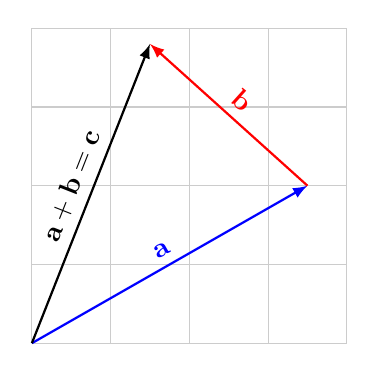
\begin{tikzpicture}[>=latex]
			\draw[thin,gray!40] (0,0) grid (4,4);
			\draw[blue,thick,->] (0,0)--(3.5,2) node[midway,above,sloped] {$\textbf{a}$};
			\draw[red,thick,->] (3.5,2)--(1.5,3.8) node[midway,above,sloped] {$\textbf{b}$};
			\draw[black,thick,->] (0,0)--(1.5,3.8)node[midway,above,sloped] {$\textbf{a} +\textbf{b} = \textbf{c} $};
		\end{tikzpicture}
		\caption{Addition von zwei Vektoren\label{figure:addition}}
\end{figure}
Was soll es schon heissen zwei Vektoren miteinander zu multiplizieren? 
Im Folgenden werden wir versuchen diese Operation ähnlich intuitiv darzustellen.

Um sinnvoll eine neue Operation zwischen zwei Elementen einer Algebra, in diesem Fall sind diese Elemente Vektoren, zu definieren, muss man überlegen, was das Ziel dieser Operation sein soll.
 
\begin{ziel}
	\label{clifford:ziel}
	Der Vektorraum der $n$-dimensionalen Vektoren soll zu einer Algebra so erweitert werden, dass das Quadrat von Vektoren durch die Länge des Vektors ausgedrückt werden kann.
\end{ziel}
Zusätzlich soll auch das Assoziativgesetz für die Multiplikation von Vektoren gelten, das heisst wir dürfen wie in
\index{Assoziativgesetz}%
\begin{equation*}
    \label{eq:assoziativ}
    \textbf{e}_i(\textbf{e}_j + \textbf{e}_k) 
    = 
    \textbf{e}_i\textbf{e}_j + \textbf{e}_i\textbf{e}_k
\end{equation*}
ausklammern.
Allerdings gilt das Kommutativgesetz leider oder, wie man sehen wird, zum Glück nur für skalare Elemente wie in
\index{Kommutativgesetz}%
\begin{equation}
    \label{eq:kommSkalar}
    a\textbf{e}_ib\textbf{e}_j 
    = 
    ab\textbf{e}_i\textbf{e}_j \qquad a,b \in \mathbb{R},
\end{equation}
aber nicht für Vektoren. Im Allgemeinen wird
\begin{equation}
    \label{eq:kommVector}
    \textbf{e}_i\textbf{e}_j 
    \neq 
    \textbf{e}_j\textbf{e}_i
\end{equation}
sein.
\subsubsection{Quadrieren eines Vektors}
\index{Quadrieren}%
Betrachten wir nun mit diesen Regeln das Quadrat eines Vektors.
Zuerst werden die Vektoren als Linearkombinationen geschrieben:
\begin{equation}
	    \textbf{a}^2 = 
		\biggl( 
		\sum_{i=1}^{n} a_i \textbf{e}_i 
		\biggr) 
		\biggl( 
		\sum_{i=1}^{n} a_i \textbf{e}_i 
		\biggr)
		\label{eq:quad_a_1}.
\end{equation}
Das Quadrat kann nun in zwei Summen 
\begin{equation}
	\textbf{a}^2 =
	\textcolor{red}{\sum_{i=1}^{n} a_i^2\textbf{e}_i^2} 
	+ 
	\textcolor{blue}{\sum_{\begin{subarray}{l}i,j=1\\i \neq j\end{subarray}}^n  a_ia_j\textbf{e}_i\textbf{e}_j } 
	\label{eq:quad_a_2}
\end{equation}
aufgeteilt werden, wobei die roten Summe die quadrierten Terme und die blaue Summe die Mischterme beinhaltet.
Wie zuvor in Ziel~\ref{clifford:ziel} definiert, ergibt das Quadrat eines Vektors dessen Länge
 Da die Basisvektoren orthonormiert sind, muss $\textbf{e}_i^2 = 1$ gelten:
\begin{equation}
	\textbf{a}^2 = \textcolor{red}{\sum_{i=1}^{n} a_i^2} + \textcolor{blue}{\sum_{\begin{subarray}{l}i,j=1\\i \neq j\end{subarray}}^n  a_ia_j\textbf{e}_i\textbf{e}_j}.
	\label{eq:quad_a_3}
\end{equation}
\begin{beispiel}
Das Quadrat des Vektor $\textbf{a}$ in $\mathbb{R}^2$ ist
\begin{align*}
    \textbf{a}^2 
    &= (a_1\textbf{e}_1+a_2\textbf{e}_2)(a_1\textbf{e}_1+a_2\textbf{e}_2) \\
    &= \textcolor{red}{a_1^2\textbf{e}_1^2 + a_2^2\textbf{e}_2^2} 
    + \textcolor{blue}{a_1\textbf{e}_1a_2\textbf{e}_2 + a_2\textbf{e}_2a_1\textbf{e}_2}   \\
    & = \textcolor{red}{a_1^2 + a_2^2} + \textcolor{blue}{a_1b\textbf{e}_1a_2\textbf{e}_2 + a_2\textbf{e}_2a_1\textbf{e}_2}.
\qedhere
\end{align*}
\end{beispiel}

Der rote Teil von \eqref{eq:quad_a_3} ist nun bereits die Länge im Quadrat, also das zuvor definierte Ziel der Multiplikation.
Daraus lässt sich schliessen, dass der restliche Teil dieser Gleichung
\begin{equation}
    \label{eq:Mischterme_Null}
    \sum_{\begin{subarray}{l}i,j=1\\i \neq j\end{subarray}}^n  a_ia_j\textbf{e}_i\textbf{e}_j  = \textcolor{blue}{a_1a_2(\textbf{e}_1\textbf{e}_2 + \textbf{e}_2\textbf{e}_1)} + a_1a_3(\textbf{e}_1\textbf{e}_3 + \textbf{e}_3\textbf{e}_1) + \dots =  0.
\end{equation}
 ergeben muss.
 Aus dieser Erkenntnis können weitere Eigenschaften für die Multiplikation hergeleitet werden.
 
Da dies für beliebige $a_i$ gelten muss, werden alle Terme bis auf $a_1$ und $a_2$ gleich null gesetzt.
Somit fallen alle Terme bis auf den blauen weg.
Wird dies weiter vereinfacht, ergibt sich
\begin{equation*}
\begin{aligned}
    a_1a_2(\textbf{e}_1\textbf{e}_2 + \textbf{e}_2\textbf{e}_1) &= 0 \\
    a_1a_2\textbf{e}_1\textbf{e}_2 &= -a_1a_2\textbf{e}_2\textbf{e}_1 \\
    \textbf{e}_1\textbf{e}_2 &= -\textbf{e}_2\textbf{e}_1.
\end{aligned}
\end{equation*}
\begin{satz}
  Die Multiplikation von orthogonalen Vektoren ist antikommutativ:
    \begin{equation*}
        \mathbf{e}_i\mathbf{e}_j = -\mathbf{e}_j\mathbf{e}_i \quad \textrm{für} \quad \mathbf{e}_i \perp \mathbf{e}_j.
    \end{equation*}
\end{satz}
Dieses Wissen reicht nun bereits, um alle Produkte der Basisvektoren zu berechnen, was in Tabelle \ref{tab:multip_vec} gemacht wurde.
\begin{table}
\begin{center}
\begin{tabular}{ |c|ccccc| } 
 \hline
  & $\textbf{e}_1$ & $\textbf{e}_2$ & $\dots$ & $\textbf{e}_{n-1}$ & $\textbf{e}_{n}$ \\
  \hline
 $\textbf{e}_1$ & 1 & $\textbf{e}_1\textbf{e}_2$ & $\dots$ & $\textbf{e}_1\textbf{e}_{n-1}$ & $\textbf{e}_1\textbf{e}_{n}$ \\
 $\textbf{e}_2$ & $-\textbf{e}_1\textbf{e}_2$ & 1 & $\dots$ & $\textbf{e}_2\textbf{e}_{n-1}$ & $\textbf{e}_2\textbf{e}_{n}$ \\
 $\vdots$ & $\vdots$ & $\vdots$ & $\ddots$ & $\vdots$ & $\vdots$ \\
 $\textbf{e}_{n-1}$ & $-\textbf{e}_1\textbf{e}_{n-1}$ & $-\textbf{e}_2\textbf{e}_{n-1}$  & $\dots$ & $1$ & $\textbf{e}_{n-1}\textbf{e}_{n}$ \\
 $\textbf{e}_{n}$ & $-\textbf{e}_1\textbf{e}_{n}$ & $-\textbf{e}_2\textbf{e}_{n}$  & $\dots$ & $-\textbf{e}_{n-1}\textbf{e}_{n}$ & 1 \\
 \hline
\end{tabular}
\end{center}
\caption{Multiplikationstabelle für Vektoren}
\label{tab:multip_vec}
\end{table}

\subsection{Multiplikation von Vektoren}
Was geschieht nun, wenn zwei beliebige Vektoren
\begin{equation*}
    \textbf{u} = 
    \sum_{i=1}^{n} u_i \textbf{e}_i 
    \quad
    \text{und}
    \quad
    \textbf{v} = \sum_{i=1}^{n} v_i \textbf{e}_i
\end{equation*}
 miteinander multipliziert werden? 
 Wieder werden die Vektoren zuerst als Linearkombinationen dargestellt und danach in zwei Summen aufgeteilt,
eine Summe mit quadrierten Termen und eine Summe mit Mischtermen
\begin{equation}
%    \begin{split}
        \textbf{u}\textbf{v} 
        =
        \biggl( 
        \sum_{i=1}^{n} u_i \textbf{e}_i
        \biggr) 
        \biggl( 
        \sum_{i=1}^{n} v_i \textbf{e}_i
        \biggr) 
        = 
        \sum_{i=1}^n u_iv_i\underbrace{\textbf{e}_i^2}_{1} 
        + \sum_{\begin{subarray}{l}i,j=1\\i \neq j\end{subarray}}^n  u_iv_j\textbf{e}_i\textbf{e}_j.
%    \end{split}
\end{equation}
Die Summe der quadrierten Terme ist bereits aus \eqref{eq:quad_a_3} bekannt,
sie ist nämlich das Skalarprodukt von $\textbf{u}$ und $\textbf{v}$.
Die Summe der Mischterme bilden etwas Neues, dass wir das äussere Produkt von $\textbf{u}$ und $\textbf{v}$ nennen.
\begin{beispiel}
    Die Multiplikation von Vektoren in $\mathbb{R}^2$ ergibt
\begin{align*}
        \textbf{u}\textbf{v} 
        &= 
        (u_1\textbf{e}_1 + u_2\textbf{e}_2)(v_1\textbf{e}_1 + v_2\textbf{e}_2) 
        = 
        u_1v_1\textbf{e}_1^2
        + 
        u_2v_2\textbf{e}_2^2 
        + 
        u_1v_2\textbf{e}_1\textbf{e}_2 
        +  
        u_2v_1\underbrace{\textbf{e}_2\textbf{e}_1}_{-\textbf{e}_1\textbf{e}_2}
        \\\ 
        &=  
        \underbrace{(u_1v_1 + u_2v_2)}_{\text{Skalarprodukt}} 
        + 
        \underbrace{(u_1v_2 - u_2v_1)\textbf{e}_1\textbf{e}_2}_{\text{Äusseres Produkt}}.
\qedhere
\end{align*}
\end{beispiel}
\subsubsection{Das äussere Produkt}
Das äussere Produkt von zwei Vektoren wird mit einem $\wedge$ dargestellt:
\begin{equation*}
    \textbf{u}\wedge \textbf{v} 
    = 
    \sum_{\begin{subarray}{l}i,j=1\\i \neq j\end{subarray}}^n  u_iv_j\textbf{e}_i\textbf{e}_j .
\end{equation*}
\begin{beispiel}
Das äusseres Produkt von zwei Vektoren in $\mathbb{R}^3$ ist
\begin{align*}
		\textbf{u} \wedge \textbf{v}
		&= 
		u_1v_2\textbf{e}_1\textbf{e}_2 
		+ 
		u_1v_3\textbf{e}_1\textbf{e}_3 
		+ 
		u_2v_2\textbf{e}_2\textbf{e}_3 
		+ 
		u_2v_1\textbf{e}_2\textbf{e}_1 
		+ 
		u_3v_1\textbf{e}_3\textbf{e}_1 
		+
		u_3v_2\textbf{e}_3\textbf{e}_2 \\\ 
		&= 
		(u_1v_2 - u_2v_1)\textbf{e}_1\textbf{e}_2 
		+ 
		(u_1v_3 - v_3u_1)\textbf{e}_1\textbf{e}_3 
		+ 
		(u_2v_3 - u_3v_2)\textbf{e}_2\textbf{e}_3.
\qedhere
\end{align*}
\end{beispiel}

Im letzten Schritt des Beispiels wurden mit Hilfe der Antikommutativität des Produkts die Vektorprodukte zusammengefasst, welche die gleichen Einheitsvektoren beinhalten.
Dieses Vorgehen kann man auch allgemein anwenden, wie in den folgenden Gleichungen \eqref{eq:u_wedge_v}--\eqref{eq:u_wedge_v_5} gezeigt werden soll.
Die Summe
\begin{align}
        \textbf{u}\wedge \textbf{v}
        &= 
        \sum_{\begin{subarray}{l}i,j=1\\i \neq j\end{subarray}}^n  
        u_iv_j\textbf{e}_i\textbf{e}_j,
        \label{eq:u_wedge_v}
        \intertext{wird in zwei verschiedene Summen}
        &= 
        \sum_{\begin{subarray}{l}i,j=1\\i < j\end{subarray}}^n u_iv_j\textbf{e}_i\textbf{e}_j 
        + 
        \sum_{\begin{subarray}{l}i,j=1\\j < i\end{subarray}}^n u_iv_j\textbf{e}_i\textbf{e}_j
        \label{eq:u_wedge_v_2}
        \intertext{aufgeteilt. 
        	Die linke Summe beinhaltet den Basisvektor mit dem höheren Index an erster Stelle und die rechte Summe diesen jeweils an zweiter Stelle.Nun werden die Indizes der zweiten Summe vertauscht, sie wird}
        &= 
        \sum_{\begin{subarray}{l}i,j=1\\i < j\end{subarray}}^n u_iv_j\textbf{e}_i\textbf{e}_j 
        + 
        \sum_{\begin{subarray}{l}i,j=1\\i < j\end{subarray}}^n u_jv_i\textbf{e}_j\textbf{e}_i.
       	\intertext{Mit Hilfe der Antikommutativität kann dies umgeformt werden zu}
        &= 
        \sum_{\begin{subarray}{l}i,j=1\\i < j\end{subarray}}^n u_iv_j\textbf{e}_i\textbf{e}_j 
        - 
        \sum_{\begin{subarray}{l}i,j=1\\i < j\end{subarray}}^n u_jv_i\textbf{e}_i\textbf{e}_j.
        \intertext{Nun können die zwei Summen wieder zu}
        \label{eq:u_wedge_v_4}
        &= 
        \sum_{\begin{subarray}{l}i,j=1\\i < j\end{subarray}}^n (u_iv_j -u_jv_i)\textbf{e}_i\textbf{e}_j
        \intertext{zusammengefasst werden. Der Koeffizient $(u_iv_j - u_jv_i)$ in der Summe ist wohlbekannt, es ist nämlich die Determinante einer $2\times2$ Matrix mit $\textbf{u}$ und $\textbf{v}$ als ihre Spalten}
        &= 
        \label{eq:u_wedge_v_5}
        \sum_{\begin{subarray}{l}i,j=1\\i < j\end{subarray}}^n \begin{vmatrix} 
        u_i & v_i \\
        u_j & v_j
    \end{vmatrix}\textbf{e}_i\textbf{e}_j.
\end{align}

Die Determinante einer $2\times2$ Matrix beschreibt die Fläche, welche von den Spaltenvektoren aufgespannt wird, wie in Abbildung \ref{figure:det} dargestellt.
\begin{figure}
	\centering
	\begin{minipage}[t]{.45\linewidth}
		\centering
		\begin{tikzpicture}[>=latex]
			\draw[thin,gray!40] (0,0) grid (4,4);
			\draw[->] (0,0)--(4.2,0) node[right]{$x$};
			\draw[->] (0,0)--(0,4.2) node[above]{$y$};
			\draw[line width=0,fill=gray!40] (0,0)--(3,1)--(4,3)--(1,2);
			\draw[line width=2pt,blue,-stealth](0,0)--(3,1) node[anchor=north
			west]{$\boldsymbol{u}$};
			\draw[line width=2pt,red,-stealth](0,0)--(1,2) node[anchor=south east]{$\boldsymbol{v}$};
			\draw[black] (2,1.5)--(1.8,3.2) node[anchor = south]{$\begin{vmatrix} 
					u_i & v_i \\
					u_j & v_j
				\end{vmatrix} = u_iv_j - v_iu_j$};
		\end{tikzpicture}
		\caption{Geometrische Interpretation der Determinante einer $2 \times 2$ Matrix\label{figure:det}}
	\end{minipage}%
	\hfill%
	\begin{minipage}[t]{.45\linewidth}
		\centering
		\begin{tikzpicture}[>=latex]
			\draw[thin,gray!40] (0,0) grid (4,4);
			\draw[->] (0,0)--(4.2,0) node[right]{$x$};
			\draw[->] (0,0)--(0,4.2) node[above]{$y$};
			\draw[line width=0,fill=gray!40] (0,0)--(3,1)--(4,3)--(1,2);
			\draw[line width=2pt,blue,-stealth](0,0)--(3,1) node[anchor=north
			west]{$\boldsymbol{u}$};
			\draw[line width=2pt,red,-stealth](0,0)--(1,2) node[anchor=south east]{$\boldsymbol{v}$};
			\draw[->] (2.15,1.5) arc (0:310:0.3);
			\draw[black] (2,1.5)--(3.3,3.2) node[anchor = south]{$u\wedge v = \begin{vmatrix} 
					u_i & v_i \\
					u_j & v_j
				\end{vmatrix} e_1e_2 = (u_iv_j - v_iu_j)\textbf{e}_1\textbf{e}_2$};
		\end{tikzpicture}
		\caption{Geometrische Interpretation des äusseren Produktes \label{figure:wedge}}
	\end{minipage}
\end{figure}
Das äussere Produkt besteht nun also aus der Summe 
    %\(\sum_{\begin{subarray}{l}i,j=1\\i < j\end{subarray}}^n\)
    von Flächen 
    \(\begin{vmatrix} 
    	u_i & v_i \\
    	u_j & v_j
    \end{vmatrix}\)
, welche in $\textbf{e}_i\textbf{e}_j$ aufgespannt sind, wie man in \eqref{eq:u_wedge_v_5} sieht. 
Dieses Produkt $\textbf{e}_i\textbf{e}_j$ der Basisvektoren interpretiert man als Umlaufrichtung.
\index{Umlaufrichtung}%
Die gebildete Fläche wird in Richtung des ersten Vektors umschritten. 
Dies ist in Abbildung \ref{figure:wedge} dargestellt, wobei bei diesem Beispiel die Umlaufrichtung im Gegenuhrzeigersinn ist, da die Fläche in Richtung $\textbf{u}$ umschritten wird. 
Diese Fläche mit einer Richtung nennt man in der geometrischen Algebra einen Bivektor, da er eine Art zweidimensionaler Vektor ist. 
\index{Bivektor}%

\subsection{Geometrisches Produkt}
\index{geometrisches Produkt}
Die Multiplikation von zwei Vektoren nennt man in der Clifford Algebra das geometrische Produkt, dieses können wir nun als Summe aus dem Skalar- und dem äusseren Produkt darstellen als
\begin{equation*}
    \textbf{u}\textbf{v} = \textbf{u}\cdot \textbf{v} + \textbf{u} \wedge \textbf{v}.
\end{equation*}
Das Additionszeichen zwischen diesen zwei Produkten mag vielleicht ein wenig eigenartig wirken, da uns das Skalarprodukt einen Skalar und das äussere Produkt einen Bivektor zurückgibt. Was bedeutet es nun also diese beiden Elemente zu addieren?
Man kann sich die Addition wie bei den komplexen Zahlen vorstellen, wobei die imaginäre Einheit auch nicht explizit zu dem reellen Teil addiert werden kann, sondern die zwei Teile zusammen ein Objekt, eine komplexe Zahl bilden. 
Dieses Objekt, also die Summe von verschiedenen Elemente der Clifford Algebra, wird Multivektor genannt.
\begin{definition}
Neben dem eindimensionalen Vektor, dem zweidimensionalen Bivektor gibt es noch höher dimensionale Vektoren, wie zum Beispiel der dreidimensionale Trivektor.
\end{definition}
\index{Trivektor}%
\begin{definition}
Skalare heissen auch Elemente vom Grad~0, Vektoren haben den Grad~1, Bivektoren den Grad~2, Trivektoren den Grad~3 usw.
\end{definition}
\begin{definition}
	Für das Produkt von Basisvektoren wird die Notation
	\begin{equation}
		e_ie_j = e_{i\!j}
	\end{equation}
	 definiert.
\end{definition}
\begin{definition}
	Die Linearkombination von Vektoren, Bivektoren und Produkten von Vektoren höheren Grades
  bildet einen Multivektor
	\begin{equation}
		M = \sum \left ( \prod a_i\textbf{e}_j \right ).
	\end{equation}
\end{definition}
Besteht eine Clifford Algebra aus $n$ Basisvektoren so hat sie $n$ Dimensionen, dies wird nicht wie in der linearen Algebra mit $\mathbb{R}^n$ sondern mit $G_n(\mathbb{R})$ beschrieben. Dies wird so geschrieben da man eine neue Algebrastruktur um die Vektoren einführt.
\index{GnR@$G_n(\mathbb{R})$}%
\index{Clifford Algebra}%
\begin{beispiel}
Allgemeiner Multivektor in $G_3(\mathbb{R})$:
\begin{equation*}
    M = a 
    + 
    \underbrace{b\textbf{e}_1 + c\textbf{e}_2 + d\textbf{e}_3}_{\text{Vektorteil}} 
    +
    \underbrace{f\textbf{e}_1\textbf{e}_2 + g\textbf{e}_1\textbf{e}_3 + h\textbf{e}_2\textbf{e}_3 }_{\text{Bivektorteil}} 
    +   
    \underbrace{k\textbf{e}_1\textbf{e}_2\textbf{e}_3}_{\text{Trivektorteil}}.
\end{equation*}
\end{beispiel}
\begin{table}
    \begin{center}
    \begin{tabular}{ |c|ccc|ccc|c| } 
     \hline
     $1$ & $\textbf{e}_1$ & $\textbf{e}_2$ &$\textbf{e}_3$ & $\textbf{e}_{12}$ & $\textbf{e}_{13}$ & $\textbf{e}_{23}$ & $\textbf{e}_{123}$\\
     \hline
     $\textbf{e}_1$ & 1 & $\textbf{e}_{12}$ & $\textbf{e}_{12}$ & $\textbf{e}_2$ & $\textbf{e}_3$ & $\textbf{e}_{123}$ & $\textbf{e}_{23}$\\
     $\textbf{e}_2$ & $-\textbf{e}_{12}$ & $1$ & $\textbf{e}_{23}$ & $-\textbf{e}_1$ & $-\textbf{e}_{123}$ & $\textbf{e}_3$ & $-\textbf{e}_{13}$\\
     $\textbf{e}_3$ & $-\textbf{e}_{13}$ & $-\textbf{e}_{23}$ & $1$ & $\textbf{e}_{123}$ & $-\textbf{e}_1$ & $-\textbf{e}_2$ & $\textbf{e}_{12}$\\
     \hline
     $\textbf{e}_{12}$ & -$\textbf{e}_2$ & $\textbf{e}_1$& $\textbf{e}_{123}$ & $-1$ & $-\textbf{e}_{23}$ & $\textbf{e}_{13}$ &  $-\textbf{e}_{3}$\\
     $\textbf{e}_{13}$ & $-\textbf{e}_{3}$ & $-\textbf{e}_{123}$ & $\textbf{e}_{1}$ & $\textbf{e}_{23}$ & $-1$ & $-\textbf{e}_{12}$ &  $\textbf{e}_{2}$\\
     $\textbf{e}_{23}$ &  $\textbf{e}_{123}$ & $-\textbf{e}_{3}$ & $\textbf{e}_{2}$ & $-\textbf{e}_{13}$ & $\textbf{e}_{12}$ & $-1$ & $-\textbf{e}_{1}$ \\
     \hline
     $\textbf{e}_{123}$ & $\textbf{e}_{23}$ & $-\textbf{e}_{13}$ & $\textbf{e}_{12}$ & $-\textbf{e}_{3}$& $\textbf{e}_{2}$ & $-\textbf{e}_{1}$ & $-1$ \\
     \hline
    \end{tabular}
    \end{center}
 	\caption{Multiplikationstabelle für $G_3(\mathbb{R})$
    \label{tab:multip}}
\end{table}
Nun, da das geometrische Produkt vollständig definiert wurde, können Multiplikationstabellen für verschiedene Dimensionen $G_n(\mathbb{R})$ erstellt werden. In Tabelle \ref{tab:multip} ist dies für  $G_3(\mathbb{R})$ gemacht.

\subsection{Polare Darstellung des geometrischen Produktes}
\index{Polardarstellung}%
Beide Teile des geometrischen Produktes lassen sich durch trigonometrische Terme beschreiben.
Das Skalarprodukt kann als 
\begin{equation*}
    \textbf{u}\cdot \textbf{v} = |\textbf{u}|\,|\textbf{v}|\cos{\alpha}
\end{equation*}
beschrieben werden, wobei $\alpha$ der Winkel zwischen $\textbf{u}$ und $\textbf{v}$ ist.

Beim äusseren Produkt wurde bereits erwähnt, dass es aus dem Produkt der Fläche des von den zwei Vektoren aufgespannten Parallelograms und einer Umlaufrichtung beschrieben wird.
Die Fläche eines Parallelograms lässt sich auch mit einen Sinus-Term
\begin{equation*}
    \textbf{u} \wedge \textbf{v}
    = 
    \sum_{i<j}
    \begin{vmatrix} 
        u_i & v_i \\
        u_j & v_j
    \end{vmatrix}\textbf{e}_i\textbf{e}_j  
    = 
    \underbrace{|\textbf{u}|\,|\textbf{v}|\sin{\alpha}}_{\text{Fläche}}\textbf{b}_1\textbf{b}_2
\end{equation*}
beschreiben.
Die Fläche des Parallelogramms liegt dabei auf der von $\textbf{b}_1$ und $\textbf{b}_2$ aufgespannten Ebene.

Nun kann man diese Terme wieder zum geometrischen Produkt
\begin{equation*}
    \textbf{u}\textbf{v}
    = 
    |\textbf{u}|\,|\textbf{v}|\cos{(\alpha)} 
    + 
    |\textbf{u}|\,|\textbf{v}|\sin{(\alpha)} \textbf{b}_1\textbf{b}_2
    = 
    |\textbf{u}|\,|\textbf{v}|(\cos{(\alpha)} + \sin{(\alpha)}\textbf{b}_1\textbf{b}_2)
\end{equation*}
vereinen.
Daraus kann geschlussfolgert werden, dass
\begin{equation}
	\textbf{u} \textbf{v}=-\textbf{v}\textbf{u} \quad \textrm{für} \quad \textbf{u}\perp \textbf{v} 
	\label{uperpv}
\end{equation}
und
\begin{equation}
	\textbf{u} \textbf{v}=\textbf{v}\textbf{u} \quad \textrm{für} \quad \textbf{u} \parallel \textbf{v} 
	\label{uparallelv}
\end{equation}
gilt.

%
% einleitung.tex -- Beispiel-File für die Einleitung
%
% (c) 2020 Prof Dr Andreas Müller, Hochschule Rapperswil
%
\section{Pauli-Matrizen}
\index{Pauli-Matrizen}%

Was ist der beste Weg um einen Computeralgorithmus für die Rechenoperationen in der Clifford-Algebra zu erstellen?
Man könnte versuchen, einen textuellen Rechner zu implementieren, der für die Elemente $\mathbf{e}_i$ hartkodierte Vereinfachungen ausführt.
\begin{beispiel}
	Der Algorithmus weiss, dass er $a\mathbf{e}_1\cdot b\mathbf{e}_1$ zu $ab\cdot1$ vereinfachen kann. Dies ermöglicht zum Beispiel die Vereinfachung
	\begin{equation*}
	3\mathbf{e}_1 \cdot 2\mathbf{e}_1 + 3\mathbf{e}_2 \quad\Rightarrow\quad 6 + 3\mathbf{e}_2
\qedhere
	\end{equation*}
\end{beispiel}
\rhead{Pauli-Matrizen}
Ein textueller Algorithmus ist aber sehr ineffizient.
Die Pauli-Matrizen bilden eine elegante und schnellere Alternative, welche für die dreidimensionale Clifford-Algebra verwendet werden können und alle Operationen aus der Clifford-Algebra gleich wie die Matrixoperationen ausführen lassen.
\begin{definition} \label{def:defPauli} 
	Die Matrizen
	\begin{align} \label{Pauli}
	\mathbf{e}_0 = E = 
	\begin{pmatrix}
	1 & 0 \\
	0 & 1
	\end{pmatrix},\quad
	\mathbf{e}_1 =
	\begin{pmatrix}
	0 & 1 \\
	1 & 0
	\end{pmatrix},\quad
	\mathbf{e}_2 =
	\begin{pmatrix}
	0 & -j \\
	j & 0
	\end{pmatrix},\quad
	\mathbf{e}_3 =
	\begin{pmatrix}
	1 & 0 \\
	0 & -1
	\end{pmatrix}	
	\end{align}
	heissen Pauli-Matrizen ($\mathbf{e}_0$ = Skalare)
\end{definition}
Die Matrix-Multiplikationen der Pauli-Matrizen führt auf die gleichen algebraischen Relationen, wie die Multiplikation der Elemente $\mathbf{e}_0, \mathbf{e}_1, \mathbf{e}_2, \mathbf{e}_3$.
So lassen sich auch die restlichen Elemente der Clifford-Algebra erzeugen.
\begin{definition} \label{def:defPauli2} 
	Die Bivektoren und Trivektoren hergeleitet aus den Pauli-Matrizen sind
	\begin{align} \label{Pauli2}
	\mathbf{e}_{12} =  
	\begin{pmatrix}
	j & 0 \\
	0 & -j
	\end{pmatrix}\quad
	\mathbf{e}_{23} =
	\begin{pmatrix}
	0 & j \\
	j & 0
	\end{pmatrix}\quad
	\mathbf{e}_{31} =
	\begin{pmatrix}
	0 & 1 \\
	-1 & 0
	\end{pmatrix}\enspace\text{und}\enspace
	\mathbf{e}_{123} =
	\begin{pmatrix}
	j & 0 \\
	0 & j
	\end{pmatrix}.
	\end{align}
\end{definition}
Dabei ist wichtig, dass sich die Matrizen gleich verhalten, wie es die Clifford-Algebra für die Basiselemente definiert hat. Zum Beispiel gilt in der Clifford-Algebra $\mathbf{e}_1^2=\mathbf{e}_0$ und $\mathbf{e}_{12}^2=-\mathbf{e}_0$, genau die selbe Relation gilt auch für die zugehörigen Matrizen, wie man durch die Matrizenrechnungen
\begin{align*}
\mathbf{e}_1^2 &=
\begin{pmatrix}
0 & 1 \\
1 & 0
\end{pmatrix}^2 = 
\begin{pmatrix}
1 & 0 \\
0 & 1
\end{pmatrix}= \mathbf{e}_0 \quad\text{und}\\
\mathbf{e}_{12}^2 &=
\begin{pmatrix}
j & 0 \\
0 & -j
\end{pmatrix}^2 = 
\begin{pmatrix}
-1 & 0 \\
0 & -1
\end{pmatrix} = -\mathbf{e}_0 
\end{align*}
bestätigt.
Man kann bei den Definitionen \ref{def:defPauli} und \ref{def:defPauli2} sehen, dass alle Matrizen linear unabhängig voneinander sind.
Das bedeutet, dass wenn man die Matrizen der Basiselemente normal addiert und zu einer Matrix zusammenfasst, kann man anschliessend die einzelnen Anteile der Basiselemente wieder herauslesen.
\begin{hilfssatz}
	Ein beliebiger Multivektor
	\begin{align} \label{MultiVektorAllg}
	M = a_0\mathbf{e}_0 + a_1\mathbf{e}_1 + a_2\mathbf{e}_3 + a_{12}\mathbf{e}_{12} + a_{23}\mathbf{e}_{23} + a_{31}\mathbf{e}_{31} + a_{123}\mathbf{e}_{123}
	\end{align}
	erhält durch das Einsetzten der Matrizen aus \eqref{Pauli} und \eqref{Pauli2} die Form
	\begin{align}
	M =
	\begin{pmatrix}
	(a_0+a_3) + (a_{12}+a_{123})j & (a_1+a_{31})+(-a_2+a_{23})j \\
	(a_1-a_{31})+(a_2+a_{23})j & (a_0-a_3)+(-a_{12}+a_{123})j
	\end{pmatrix}.\label{MultivektorMatirx}
	\end{align}
\end{hilfssatz}
Die Anteile treten zudem immer paarweise auf und können somit immer je durch zwei Gleichungen bestimmt werden.
\begin{beispiel}
	Die Matrix
	\begin{equation*}
	M = 
	\begin{pmatrix}
	1 & 0 \\
	0 & -1j
	\end{pmatrix}
	\end{equation*}
	soll als Multivektor in der Form \eqref{MultiVektorAllg} geschrieben werden. Dafür entnehmen wir aus \eqref{MultivektorMatirx} die Gleichungen
	\begin{equation*}
	a_0 + a_3 = 1,\quad a_0 - a_3 = 0,\quad a_{12}+a_{123} = 0\enspace\text{und}\enspace -a_{12}+a_{123}=-1,
	\end{equation*}
	aus denen man auf
	\begin{equation*}
	a_0 = \dfrac{1}{2},\quad a_3 = \dfrac{1}{2},\quad a_{12}=\dfrac{1}{2}\enspace\text{und}\enspace a_{123}=-\dfrac{1}{2}
	\end{equation*}
	schliessen kann. Da die restlichen Realteile und Imaginärteile 0 sind, werden die anderen Anteile ebenfalls 0 sein. Daher ist
	\begin{equation*}
	M = \dfrac{1}{2} \mathbf{e}_0+ \dfrac{1}{2} \mathbf{e}_3 + \dfrac{1}{2} \mathbf{e}_{12} - \dfrac{1}{2} \mathbf{e}_{123}.
\qedhere
	\end{equation*}
\end{beispiel}
Die Clifford-Algebra ist bei der Darstellung durch Matrizen kein Ausnahmefall. Es lässt sich theoretisch jede algebraische Struktur durch Matrizen darstellen.

%
% teil1.tex -- Beispiel-File für das Paper
%
% (c) 2020 Prof Dr Andreas Müller, Hochschule Rapperswil
%
\section{Spiegelung}
\rhead{Spiegelung}

Die Spiegelung ist eine grundlegende, geometrische Operation, aus welcher man weitere Operationen, wie beispielsweise die später beschriebene Drehung, ableiten kann. Da die geometrische Algebra für geometrische Anwendungen ausgelegt ist, sollte die Spiegelung auch eine einfache, praktische Formulierung besitzen.
\begin{figure}
	\centering
	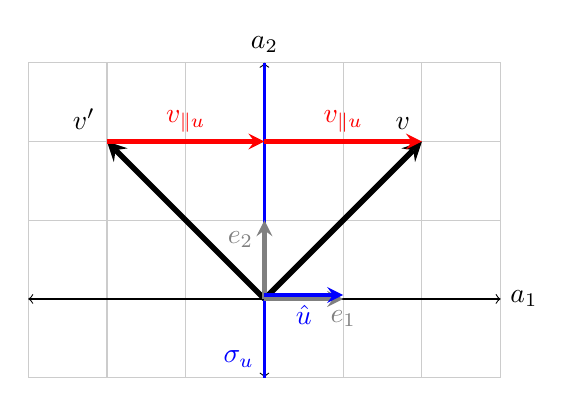
\begin{tikzpicture}
	\draw[thin,gray!40] (-3,-1) grid (3,3);
	\draw[<->] (-3,0)--(3,0) node[right]{$a_1$};
	\draw[<->] (0,-1)--(0,3) node[above]{$a_2$};
	\draw[blue, line width=1.0pt] (0,3)--(0,-1) node[anchor=south east]{$\sigma_u$};
	\draw[line width=2pt,black,-stealth](0,0)--(2,2) node[anchor=south east]{$\boldsymbol{v}$};
	\draw[line width=2pt,black,-stealth](0,0)--(-2,2) node[anchor=south east]{$\boldsymbol{v'}$};
	\draw[line width=1.5pt,gray,-stealth](0,0)--(1,0) node[anchor=north]{$\boldsymbol{e_1}$};
	\draw[line width=1.5pt,gray,-stealth](0,0)--(0,1) node[anchor=north east]{$\boldsymbol{e_2}$};
	\draw[line width=1.5pt,red,-stealth](0,2)--(2,2) node[xshift=-1cm, yshift=
	0.25cm]{$\boldsymbol{v_{\parallel u}}$};
	\draw[line width=1.5pt,red,-stealth](-2,2)--(0,2) node[xshift=-1cm, yshift=
	0.25cm]{$\boldsymbol{v_{\parallel u}}$};
	\draw[line width=1.5pt,blue,-stealth](0,0.05)--(1,0.05) node[xshift=-0.5cm, yshift=-0.25cm]{$\boldsymbol{\hat{u}}$};
	\end{tikzpicture}
	\caption{Spiegelung des Vektors $\mathbf{v}$ an der Spiegelebene $\sigma_u$ mit dem Normalenvektor $\mathbf{\hat{u}}$}
	\label{BildSpiegelung}
\end{figure}

\subsection{Linearen Algebra}
Aus der linearen Algebra ist bekannt, dass man eine Spiegelung an einer Ebene, wie in Abbildung \ref{BildSpiegelung} gezeigt, wie folgt beschreiben kann.
\begin{definition}
	Die Abbildung der Spiegelung in der linearen Algebra mit dem Normalenvektor $\mathbf{\hat{u}}$ zur Spiegelebene ist
	\begin{equation} \label{RefLinAlg}
	\mathbf{v} = \mathbf{v_{\perp u}} + \mathbf{v_{\parallel u}} \enspace\mapsto\enspace \mathbf{v'} =  \mathbf{v_{\perp u}} - \mathbf{v_{\parallel u}} = \mathbf{v} - 2 \cdot \mathbf{v_{\parallel u}}.
	\end{equation}
\end{definition}
Es scheint für diese Formel \eqref{RefLinAlg} aber umständlich zu sein, weitere Spiegelungen mit weiteren Spiegelebenen anzufügen. Weil man $\mathbf{v_{\parallel u}}$ auch als Skalarprodukt $\mathbf{v_{\parallel u}} = \mathbf{\hat{u}} \cdot \mathbf{v}$ schreiben kann, ist es leicht diese Abbildung auch als Matrix darzustellen. Sei $\mathbf{\hat{u}}$ ein Normalenvektor auf die Spiegelungsebene, also $\mathbf{\hat{u}}\perp \sigma_u$, und sei ausserdem normiert $|\mathbf{\hat{u}}| = 1$, dann kann man die Spiegelung durch die Matrix
\begin{align}
S = E - 2\mathbf{\hat{u}\hat{u}}^t
\end{align}
beschrieben werden. In zwei und drei Dimensionen ergibt die Berechnung
\begin{align} \label{Spiegelmatrizen}
S_2 = \begin{pmatrix}
1-2u_1^2 & -2u_1u_2 \\
-2u_1u_2 & 1-2u_2^2
\end{pmatrix}\quad\text{und}\quad
S_3 = \begin{pmatrix}
1-2u_1^2 & -2u_1u_2 & -2u_1u_3\\
-2u_1u_2 & 1-2u_2^2 & -2u_2u_3\\
-2u_1u_3 & -2u_2u_3 & 1-2u_3^2\\
\end{pmatrix}.
\end{align}
Diese Spiegelmatrizen gehören der orthogonalen Matrizengruppe $S_n\in \text{O}(n)$ an. Die Matrizengruppe $\text{O}(n)$ hat die Eigenschaft $S_n^t S_n = E$, was bedeutet, dass die Länge und Winkel bei der Abbildung beibehalten bleiben. Zusätzlich sind die Spiegelmatrizen symmetrisch, es gilt $S_n^t = S_n$. Somit liefert zweimal dieselbe Spiegelung wieder die identische Abbildung, wie man aus
\begin{align}
S_n^t S_n = S_n^2 = E
\end{align}
schliessen kann.

\subsection{Geometrische Algebra}
Wir definieren zuerst die Inverse eines Vektors, welche in dieser Form nicht in der linearen Algebra nicht existiert.
\begin{definition}
	Die Inverse eines Vektors wird definiert als
	\begin{align} \label{InverseGA}
	\mathbf{u}^{-1} = \dfrac{\mathbf{u}}{|\mathbf{u}|^2}. 
	\end{align}
\end{definition}
Diese Definition ist sinnvoll, da wegen $\mathbf{u}^2 = |\mathbf{u}|^2$ folgt
\begin{align}
\mathbf{uu}^{-1} = \mathbf{u} \frac{\mathbf{u}}{|\mathbf{u}|^2} = \frac{\mathbf{u}^2}{|\mathbf{u}|^2} = \frac{|\mathbf{u}|^2}{|\mathbf{u}|^2} = 1.
\end{align}
Der Vektor $\mathbf{u}^{-1}$ in \eqref{InverseGA} ist also tatsächlich das inverse Element im Sinne des Produktes in der geometrischen Algebra.
Die geometrische Algebra leitet aus der obigen Formel \eqref{RefLinAlg} für eine Spiegelung eine einfache und intuitive Form her, welche auch für weitere Operationen erweitert werden kann.
\begin{definition}
	Die Abbildung der Spiegelung in der geometrischen Algebra mit dem senkrechten Vektor $\mathbf{u}$ zur Spiegelungsebene $\sigma_u$ ist 
	\begin{align}\label{RefGA}
	\mathbf{v} \enspace\mapsto\enspace \mathbf{v}' = -\mathbf{uvu}^{-1}
	\end{align}
\end{definition}
Um zu überprüfen, ob die Spiegelungsgleichung \eqref{RefGA} wirklich eine Spiegelung ist, setzen wir zuerst in diese Gleichung $\mathbf{v} = \mathbf{v_{\perp u}} + \mathbf{v_{\parallel u}}$ ein. Wir bekommen somit
\begin{align}
\mathbf{v}' = -\mathbf{uv_{\perp u}u}^{-1} - \mathbf{uv_{\parallel u}u}^{-1}.
\end{align}
Danach können wir mit Hilfe der aus der Schlussfolgerung \eqref{uperpv} und \eqref{uparallelv} hergeleiteten Zusammenhänge
\begin{align}
\mathbf{uv_{\perp u}} = -\mathbf{v_{\perp u}u} \quad\text{und}\quad \mathbf{uv_{\parallel u}}=\mathbf{v_{\parallel u}u},
\end{align}
die Gleichung weiter umformen zu
\begin{align}
\mathbf{v}' = -(-\mathbf{v_{\perp u}}\underbrace{\mathbf{u})\mathbf{u}^{-1}}_{1} -(\mathbf{v_{\parallel u}}\underbrace{\mathbf{u})\mathbf{u}^{-1}}_{1} = \mathbf{v_{\perp u}} - \mathbf{v_{\parallel u}}.
\end{align}
Man sieht, dass das Resultat $\mathbf{v}' = \mathbf{v_{\perp u}} - \mathbf{v_{\parallel u}}$
gleichbedeutend zu der Definition \eqref{RefLinAlg} der Spiegelung ist.

Verwendet man für $\mathbf{u}$ nur einen Einheitsvektor $\mathbf{\hat{u}}$, welcher die Länge 1 besitzt, wird die Gleichung \eqref{RefGA} zu
\begin{align}
\mathbf{v'} = -\mathbf{\hat{u}v\hat{u}}
\end{align}
vereinfacht. Im Gegensatz zu den Abbildungen in der linearen Algebra, welche in jeder anderen Dimension, durch andere Matrizen \eqref{Spiegelmatrizen} beschrieben werden müssen, ist es in der geometrischen Algebra immer der gleiche Vorgehensweise. Zudem ist diese kompakte Schreibweise in der linearen Algebra nicht möglich, da bis auf das Vektorprodukt in drei Dimensionen keine Multiplikation von Vektoren definiert ist. 
%
% teil2.tex -- Beispiel-File für teil2 
%
% (c) 2020 Prof Dr Andreas Müller, Hochschule Rapperswil
%
\section{Drehung}
\rhead{Drehung}

Eine Drehung kann man aus zwei aufeinanderfolgenden Spiegelungen bilden. Das kann vielleicht zuerst eine verwirrende Aussage sein, da man aus den vorherig gezeigten Formeln annehmen könnte, dass die Spiegelung schon für eine Drehung ausreicht. Obwohl sich die Längen, Winkel und Volumen sich bei einer Spiegelung, wie bei einer Drehung, nicht ändert, sind sie doch verschieden, da die Orientierung bei der Spiegelung invertiert wird. Stellt man sich, wie im Bild \ref{BildSpiegRot} dargestellt, beispielsweise ein Objekt vor und spiegelt dieses an einer Ebene, dann ist es unmöglich, nur durch eine Drehung (egal an welchem Punkt) das ursprüngliche Objekt deckungsgleich auf das Gespiegelte zu drehen. Hingegen ist es wiederum möglich ein zweifach gespiegeltes Objekt durch eine Drehung zu erreichen. Das liegt daran, da die Orientierung zweimal invertiert wurde.

\begin{figure}
	\centering
	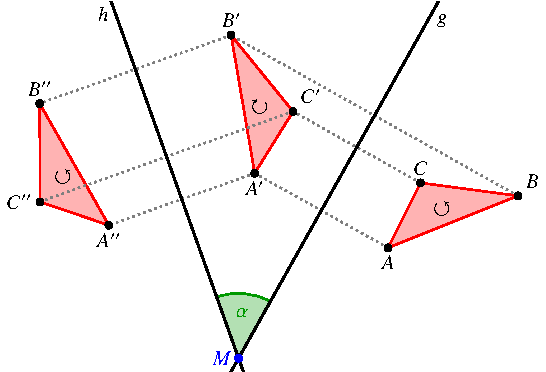
\includegraphics[width=10cm]{papers/clifford/images/spiegelung.pdf}
	\caption{Der wesentliche Unterschied zwischen Spiegelung und Drehung ist die Umkehrung der Orientierung}
	\label{BildSpiegRot}
\end{figure}

\begin{figure}
	\centering
	\begin{tikzpicture}
	\draw[thin,gray!40] (-3,-1) grid (3,3);
	\draw[<->] (-3,0)--(3,0) node[right]{$a_1$};
	\draw[<->] (0,-1)--(0,3) node[above]{$a_2$};
	\draw[line width=1.0pt,green,-stealth](2,2)--(-2,2) node[anchor=south west]{$\boldsymbol{-2v_{\parallel u}}$};
	\draw[line width=1.0pt,green,-stealth](-2,2)--(-2.828,0) node[anchor=north west]{$\boldsymbol{-2v'_{\parallel w}}$};
	\draw[blue, line width=1.0pt] (0,3)--(0,-1) node[anchor=south east]{$\sigma_u$};
	\draw[red, line width=1.0pt] (-3,1.24)--(2.21,-1) node[anchor=south]{$\sigma_w$};
	\draw[line width=2pt,black,-stealth](0,0)--(2,2) node[anchor=south east]{$\boldsymbol{v}$};
	\draw[line width=1.5pt,blue,-stealth](0,0)--(2.5, 0) node[anchor=south east]{$\boldsymbol{u}$};
	\draw[line width=2pt,black,-stealth](0,0)--(-2,2) node[anchor=south east]{$\boldsymbol{v'}$};
	\draw[line width=1.5pt,red,-stealth](0,0)--(0.957, 2.31) node[anchor=south east]{$\boldsymbol{w}$};
	\draw[line width=2pt,black,-stealth](0,0)--(-2.828,0) node[anchor=south east]{$\boldsymbol{v''}$};
	\draw[line width=1.5pt,gray,-stealth](0,0)--(1,0) node[anchor=north]{$\boldsymbol{e_1}$};
	\draw[line width=1.5pt,gray,-stealth](0,0)--(0,1) node[anchor=north east]{$\boldsymbol{e_2}$};
	
	\coordinate (A) at (0,0);
	\coordinate (B) at (2.5,0);
	\coordinate (C) at (0.957, 2.31);
	\tikzset{anglestyle/.style={angle eccentricity=1.25, purple, draw,  thick, angle radius=1cm}}
	\draw pic ["$\theta$", anglestyle] {angle = B--A--C};
	\coordinate (D) at (0,0);
	\coordinate (E) at (1,1);
	\coordinate (F) at (-1, 0);
	\tikzset{anglestyle/.style={angle eccentricity=1.25, purple,  draw,  thick, angle radius=1.25cm}}
	\draw pic ["$2\theta$", anglestyle] {angle = E--D--F};
	\end{tikzpicture}
	\caption{Drehung des Vektors $\textbf{v}$ um $2\theta$}
	\label{BildDrehung}
\end{figure}

\subsection{Linearen Algebra}
In der linearen Algebra haben wir Drehungen durch die Matrizen der Gruppe $\text{SO}(n)$ beschrieben. Beispielsweise besteht $\text{SO}(2)$  aus den Matrizen
\begin{align}
D = 
\begin{pmatrix}
\cos(\alpha) & \sin(\alpha) \\
-\sin(\alpha) & \cos(\alpha) 
\end{pmatrix},\quad
\alpha \in [0, 2\pi).
\end{align}
Diese Drehmatrizen gehören der speziellen orthogonalen Matrizengruppe $D\in \text{SO}(n) = \text{SL}_n(\mathbb{R})\enspace \cap \enspace \text{O}(n)$ an. $\text{SL}_n(\mathbb{R})$ beinhaltet die Matrizen mit scherenden Eigenschaften. Die Drehmatrizen haben die Eigenschaft $D^t D = E \enspace \land \enspace \det(D)=1$. Da $\det(D) = 1$ und nicht $-1$ sein kann fallen alle Spiegelungen aus der Menge heraus. $\det(D) = -1$ bedeutet, dass eine Orientierungsinversion stattfindet. Eine übersichtliche Darstellung der beschriebenen Matrizengruppen sieht man in der Abbildung \ref{BildMatrizenGruppen}

\begin{figure}
	\centering
	\includegraphics[width=10cm]{papers/clifford/Bilder/MatrizenGruppen.png}
	\caption{Matrizengruppen}
	\label{BildMatrizenGruppen}
\end{figure}

\subsection{Geometrische Algebra}
Da wir jetzt aus der Geometrie wissen, dass eine Drehung durch zwei Spiegelungen gebildet werden kann, können wir die Drehung mit der Formel \eqref{RefGA} einfach herleiten.
\begin{satz}
	Durch zwei nacheinander auf einen Vektor $\mathbf{v}$ angewendete Spiegelungen lässt sich eine Drehung 
	\begin{align} \label{rotGA}
	\mathbf{v}'' = -\mathbf{wv}'\mathbf{w}^{-1} = -\mathbf{w}(-\mathbf{uvu}^{-1})\mathbf{w}^{-1} = (\mathbf{wu})\mathbf{v}(\mathbf{u}^{-1}\mathbf{w}^{-1})
	\end{align}
	beschreiben.
\end{satz}
Die Vektoren $\mathbf{w}$ und $\mathbf{u}$ bilden hier wiederum die Spiegelachsen. Diese Formel versuchen wir jetzt noch durch Umstrukturierung zu verbessern. 
\subsubsection{Exponentialform}
Dazu leiten wir zuerst die Exponentialform eines Vektors her. Es wird dabei zur Vereinfachung davon ausgegangen, dass alle Vektoren $\mathbf{w}, \mathbf{u}, \mathbf{v}$ in der $\mathbf{e}_{1}$-$\mathbf{e}_{2}$-Ebene liegen. Weitere Drehungen können in höheren Dimensionen durch Linearkombinationen von Drehungen in den $\mathbf{e}_{i}$-$\mathbf{e}_{j}$-Ebenen $(i\not=j)$ erreicht werden. Für die Herleitung ersetzen wir als erstes in der Polarform
\begin{align}
\mathbf{w} = |\mathbf{w}| \left(\cos(\theta_w) \mathbf{e}_1 + \sin(\theta_w) \mathbf{e}_2\right)
\end{align}
eines Vektors einen Faktor 1 durch $1=\mathbf{e}_1^2$ und erhalten beim Sinus
\begin{align}\label{e1ausklammern}
\mathbf{w} &= |\mathbf{w}| \left(\cos(\theta_w) \mathbf{e}_1 + \sin(\theta_w) \mathbf{e}_1\mathbf{e}_1\mathbf{e}_2\right). 
\end{align}
In einem zweiten Schritt klammern wir $\mathbf{e}_1$ aus, dies ergibt
\begin{align}
\mathbf{w} = |\mathbf{w}|\mathbf{e}_1\left(\cos(\theta_w)+ \sin(\theta_w) \mathbf{e}_{12}\right). \label{ExponentialGA}
\end{align}
Die Ähnlichkeit des Klammerausdrucks in der Formel \eqref{ExponentialGA} zu der Eulerschen Formel bei den komplexen Zahlen ist nun schon gut erkennbar. Versuchen wir nun mithilfe der Reihenentwicklungen
\begin{align}
\sin(\theta_w)\mathbf{e}_{12}&=\sum _{n=0}^{\infty }(-1)^{n}{\frac {\theta_w^{2n+1}}{(2n+1)!}}\mathbf{e}_{12} =\theta_w\mathbf{e}_{12}-{\frac {\theta_w^{3}}{3!}}\mathbf{e}_{12}+{\frac {\theta_w^{5}}{5!}}\mathbf{e}_{12}-\cdots \\
\cos(\theta_w)&=\sum _{n=0}^{\infty }(-1)^{n}{\frac {\theta_w^{2n}}{(2n)!}} =1-{\frac {\theta_w^{2}}{2!}}+{\frac {\theta_w^{4}}{4!}}-\cdots
\end{align}
diesen Zusammenhang auch hier herzustellen. Setzt man diese beiden Reihenentwicklungen in \eqref{ExponentialGA} ein, erhält man
\begin{align}
\cos(\theta_w)+ \sin(\theta_w) \mathbf{e}_{12} &= 1+\theta_w\mathbf{e}_{12}-{\frac {\theta_w^{2}}{2!}}-{\frac {\theta_w^{3}}{3!}}\mathbf{e}_{12}+{\frac {\theta_w^{4}}{4!}}+{\frac {\theta_w^{5}}{5!}}\mathbf{e}_{12}-\cdots
\end{align}
Dies sieht noch nicht wie eine Exponentialreihe aus, da $\mathbf{e}_{12}$ nur in jedem zweiten Term auftritt. Da aber $\mathbf{e}_{12}=-1$ gibt, erhält man für
\begin{align}
e^{\theta_w\mathbf{e}_{12}} = 1 \mathbf{e}_{12}^0+\theta_w\mathbf{e}_{12}^1+{\frac {\theta_w^{2}}{2!}}\mathbf{e}_{12}^2+{\frac {\theta_w^{3}}{3!}}\mathbf{e}_{12}^3+{\frac {\theta_w^{4}}{4!}}\mathbf{e}_{12}^4+{\frac {\theta_w^{5}}{5!}}\mathbf{e}_{12}^5+\cdots
\label{ExponentialGA2}
\end{align}
Man sieht, dass die beiden Reihen übereinstimmen. Es folgt somit
\begin{align}\label{EulerGA}
e^{\theta_w \mathbf{e}_{12}} = \cos(\theta_w)+ \sin(\theta_w) \mathbf{e}_{12},
\end{align} 
was zeigt, dass es eine Euler-Formel mit $\mathbf{e}_{12}$ anstelle der imaginären Einheit $j$ gibt.

Wenn man jetzt den Vektor \eqref{ExponentialGA} durch die eulersche Schreibweise
\begin{align}
\mathbf{w} = |\mathbf{w}|\mathbf{e}_1e^{\theta_w\mathbf{e}_{12}}
\end{align}
ersetzt, kann die Exponentialform des Vektors ähnlich wie die der komplexen Zahlen interpretieren. Der Einheitsvektor $\mathbf{e}_1$ wird um die Länge $|\mathbf{w}|$ gestreckt und um $\theta_w$ gedreht.
\subsubsection{Vektormultiplikation}
Nun werden wir das Vektorprodukt
\begin{align} \label{VektorproduktformelGA}
\mathbf{wu} = |\mathbf{w}|\mathbf{e}_1 e^{\theta_w \mathbf{e}_{12}}|\mathbf{u}|\mathbf{e}_1 e^{\theta_u \mathbf{e}_{12}}
\end{align}
so umformen, dass wir die Drehung nur durch Exponentialterme beschreiben können. Wir tauschen dafür zuerst beim Vektor $\mathbf{w}$ die Reihenfolge von 
$\mathbf{e}_1$ mit dem Exponentialterm $e^{\theta_w \mathbf{e}_{12}}$, indem wir bei der Gleichung \eqref{e1ausklammern} $1=\mathbf{e}_1^2$ an einer anderen Position einsetzten. Wir erhalten
\begin{align} 
\mathbf{w} &= |\mathbf{w}|\left(\cos(\theta_w)+ \sin(\theta_w) \mathbf{e}_2\mathbf{e}_1\right)\mathbf{e}_1.
\end{align}
Mithilfe der Formel \eqref{EulerGA} und dem Wissen, dass $\mathbf{e}_{21}= -\mathbf{e}_{12}$ können wir die Umformung
\begin{align}
|\mathbf{w}|e^{-\theta_w \mathbf{e}_{12}}\mathbf{e}_1
\end{align}
ausführen. Diese wichtige Umstrukturierung können wir wieder in die Vektorproduktformel \eqref{VektorproduktformelGA} einsetzen un erhalten
\begin{align}
\mathbf{wu} &= |\mathbf{w}|\,|\mathbf{u}|e^{-\theta_w \mathbf{e}_{12}}\mathbf{e}_1\mathbf{e}_1 e^{\theta_u \mathbf{e}_{12}}\\
&= |\mathbf{w}|\,|\mathbf{u}|e^{(\theta_u-\theta_w) \mathbf{e}_{12}}.
\end{align}
Das inverse Vektorprodukt
\begin{align}
\mathbf{u}^{-1}\mathbf{w}^{-1} = \dfrac{1}{|\mathbf{w}|\,|\mathbf{u}|}e^{(\theta_w-\theta_u) \mathbf{e}_{12}}
\end{align}
kann durch die selbe Methode vereinfacht werden.
Wenn wir den Winkel zwischen den Vektoren  $\mathbf{w}$ und $\mathbf{u}$ als $\theta = \theta_w - \theta_u$ definieren erhalten wir als endgültige Form der Vektorprodukte
\begin{align}\label{wuExpo}
\mathbf{wu} &= |\mathbf{w}|\,|\mathbf{u}|e^{-\theta \mathbf{e}_{12}}\enspace\text{und}\\
\mathbf{u}^{-1}\mathbf{w}^{-1} &= \dfrac{1}{|\mathbf{w}|\,|\mathbf{u}|}e^{\theta \mathbf{e}_{12}} \label{wuExpoInv}.
\end{align}
\subsubsection{Umstrukturierte Drehungsgleichung}
Setzten wir nun unsere neuen Erkenntnisse in die Gleichung \eqref{rotGA} ein, erhalten wir
\begin{align}
\mathbf{v''} = (|\mathbf{w}|\,|\mathbf{u}|e^{-\theta \mathbf{e}_{12}})\mathbf{v}\biggl(\dfrac{1}{|\mathbf{w}|\,|\mathbf{u}|}e^{\theta \mathbf{e}_{12}}\biggr)
\end{align}
und können durch die Kürzungen der Längen die vereinfachte Drehungsgleichung
\begin{align} \label{GAvereinfRot}
\mathbf{v''} = e^{-\theta \mathbf{e}_{12}} v e^{\theta \mathbf{e}_{12}}
\end{align}
bilden. Wir wissen nun, dass das diese beidseitige Multiplikation die Länge von $\mathbf{v}$ nicht verändert, da sich die Längen von $\mathbf{w}$ und $\mathbf{u}$ kürzen. Betrachten wir nun den Effekt der Exponentialterme auf $\mathbf{v}$. Dabei teilen wir den Vektor $\mathbf{v}$ auf in einen Anteil $\mathbf{v_\parallel}$, welcher auf der Ebene $\mathbf{e}_{12}$ liegt, und einen Anteil $\mathbf{v_\perp}$, welcher senkrecht zu der Ebene steht. Wir bekommen durch Einsetzten nun diese Form
\begin{align} \label{RotAufPerpPar}
\mathbf{v}'' = e^{-\theta \mathbf{e}_{12}} (\mathbf{v_\perp + v_\parallel}) e^{\theta \mathbf{e}_{12}} = e^{-\theta \mathbf{e}_{12}} \mathbf{v_\perp} e^{\theta \mathbf{e}_{12}} + e^{-\theta \mathbf{e}_{12}} \mathbf{v_\parallel} e^{\theta \mathbf{e}_{12}}.
\end{align}
Auf eine allgemeine Herleitung wird hier zwar verzichtet, aber man kann zeigen, dass man die Reihenfolge der Vektoranteile $\mathbf{v_\perp}$ und $\mathbf{v_\parallel}$ mit dem Exponentialterm $e^{-\theta \mathbf{e}_{12}}$ so vertauschen kann, dass sich 
\begin{align}
\mathbf{v}'' = \mathbf{v_\perp} e^{-\theta \mathbf{e}_{12}}  e^{\theta \mathbf{e}_{12}} +  \mathbf{v_\parallel} e^{-(-\theta) \mathbf{e}_{12}} e^{\theta \mathbf{e}_{12}}
\end{align}
ergibt. Der Winkel wird beim parallelen Anteil negiert. An der Zusammengefassten Gleichung
\begin{align}\label{RotParPerp}
\mathbf{v}'' = \mathbf{v_\perp} +  \mathbf{v_\parallel} e^{2\theta \mathbf{e}_{12}}
\end{align}
kann man sehen, dass nur der parallele Anteil $\mathbf{v_\parallel}$ des Vektors $\mathbf{v}$ auf der Ebene $\mathbf{e}_{12}$ um $2\theta$ gedreht wird. Der senkrechte Anteil $\mathbf{v_\perp}$ bleibt gleich. Wichtig dabei zu sehen ist, dass nur der Winkel zwischen den Vektoren $\mathbf{w}$ und $\mathbf{u}$ von Bedeutung ist. Die Länge und Richtung der einzelnen Vektoren spielt keine Rolle. Zeigen wir nun diese Eigenschaften an einem Beispiel
\begin{beispiel} 
	Gegeben sei ein Vektor $\mathbf{v} = 1\mathbf{e}_1 + 2\mathbf{e}_2 + 3\mathbf{e}_3$ mit zur $\mathbf{e}_{12}$-Ebene parallelen Anteil $\mathbf{v_\parallel} = 1\mathbf{e}_1 + 2\mathbf{e}_2$ und senkrechten Anteil $\mathbf{v_\perp} = 3\mathbf{e}_3$. Zusätzlich sind die Spiegelachsen $\mathbf{u} = \mathbf{e}_1$ und $\mathbf{w} = 2\mathbf{e}_2$ gegeben. Gesucht ist der rotierte Vektor $\mathbf{v}''$. Bestimmen wir als erstes das Vektorprodukt
	\begin{align}
	\mathbf{wu} = (2\mathbf{e}_2)(\mathbf{e}_1) = -2\mathbf{e}_{12}
	\end{align}
	und das Produkt der Inversen
	\begin{align}
	\mathbf{u}^{-1}\mathbf{w}^{-1} = \biggl(\dfrac{\mathbf{e}_1}{1^2}\biggr) \left(\dfrac{2\mathbf{e}_2}{2^2}\right) = \dfrac{1}{2}\mathbf{e}_{12}.
	\end{align}
	Den gedrehten Vektor $\mathbf{v}''$ können wir nun durch Einsetzen und Auflösen der Produkte in die Gleichung \eqref{rotGA} bestimmen. Der Rechnenvorgang ist
	\begin{align}
	\mathbf{v}'' = (\mathbf{wu})\mathbf{v}(\mathbf{u}^{-1}\mathbf{w}^{-1}) &= (-2e_{12})(1\mathbf{e}_1 + \mathbf{e}_2 + 1\mathbf{e}_3)(\textstyle{\frac{1}{2}}\mathbf{e}_{12})\\
	&= (2\mathbf{e}_2-2\mathbf{e}_1-2\mathbf{e}_{123})(\textstyle{\frac{1}{2}}\mathbf{e}_{12})\\
	&= -1\mathbf{e}_1 - 1\mathbf{e}_2 + 1\mathbf{e}_3.
	\end{align}
	Aus dem Resultat $\mathbf{v}''= -1\mathbf{e}_1 + 1\mathbf{e}_2 + 1\mathbf{e}_3$ können wir bestätigen, dass
	\begin{itemize}
		\item die Länge $|\mathbf{v}| = \sqrt{3}$ zur Länge $|\mathbf{v}''|=\sqrt{3}$ gleich blieb.
		\item sich der parallele Anteil $\mathbf{v_\parallel}'' = -1\mathbf{e}_1 - 1\mathbf{e}_2$ gedreht hat und der senkrechte Anteil $\mathbf{v_\perp}'' = 1\mathbf{e}_3$ unverändert blieb.
		\item der parallele Teil sich genau um $2\theta=180$° gedreht hat. $\theta$ kann übrigens durch die Umformung des Produkt $\mathbf{wu}$ in die Exponentialschreibweise
		\begin{align}
		&\mathbf{wu} = -2\mathbf{e}_{12} = 2(0-1\mathbf{e}_{12})=2(\cos\biggl(\dfrac{-\pi}{2}\biggr) + \sin\biggl(\dfrac{-\pi}{2}\biggr)\mathbf{e}_{12}) = 2e^{(-\pi/2)\mathbf{e}_{12}}
		\end{align}
		durch einen Vergleich mir der Formel \eqref{wuExpo}
		\begin{align}
		\theta = -\biggl(\dfrac{-\pi}{2}\biggr) = \dfrac{\pi}{2}
		\end{align}
		ausgelesen werden. \qedhere
	\end{itemize}
\end{beispiel} 
%
% teil3.tex -- Beispiel-File für Teil 3
%
% (c) 2020 Prof Dr Andreas Müller, Hochschule Rapperswil
%
\section{Komplexe Zahlen}
\rhead{Komplexe Zahlen}

Die komplexen Zahlen finden eine Vielzahl von Anwendungsgebiete in den Ingenieurwissenschaften. Das liegt daran, weil die komplexen Zahlen Drehungen und Schwingungen gut beschreiben können. Nach dem vorherigen Abschnitt ist es nicht überraschend, dass es möglich ist, komplexe Zahlen in der geometrischen Algebra darzustellen. Sie können durch die geraden Grade der zweidimensionalen geometrischen Algebra vollständig beschrieben werden: $\mathbf{g}_n \in G_2^+(\mathbb{R}) \cong \mathbb{C}$. Das bedeutet, eine komplexe Zahl 
\begin{equation*}
\begin{aligned}
a_0 + a_1 j &\cong a_0 + a_1 \mathbf{e}_{12} = \mathbf{g}_n,&&& a_0, a_1 &\in \mathbb{R}\\
|r|e^{\vartheta j} &\cong |r|e^{\vartheta \mathbf{e}_{12}} = \mathbf{g}_n,&&& r, \vartheta &\in \mathbb{R}
\end{aligned}
\end{equation*}
kann durch einen Skalar (Grad 0) und einen Bivektor (Grad 2) dargestellt werden, weil $j$ und $\mathbf{e}_{12}$ beide die Eigenschaft
\begin{align*}
j^2 = -1\qquad\Leftrightarrow\qquad\mathbf{e}_{12}^2 = -1
\end{align*}
besitzen. Die Kommutativität
\begin{align*}
\begin{split}
\mathbf{g}_1\mathbf{g}_2 = \mathbf{g}_2\mathbf{g}_1 \enspace&\Leftrightarrow\enspace (a + b \mathbf{e}_{12})(f + g \mathbf{e}_{12}) = (f + g \mathbf{e}_{12})(a + b \mathbf{e}_{12})\\ &\Leftrightarrow\enspace |\mathbf{g}_1|\,|\mathbf{g}_2|e^{(\vartheta_{g_1} + \vartheta_{g_2})\mathbf{e}_{12}} =  |\mathbf{g}_2|\,|\mathbf{g}_1|e^{(\vartheta_{g_2} + \vartheta_{g_1})\mathbf{e}_{12}},
\end{split}
\end{align*}
welche wir schon von den komplexen Zahlen her kennen, ist dabei eine in der geometrischen Algebra nur selten anzutreffende Eigenschaft. Beispielsweise ist das geometrische Produkt 
\begin{align*}
\mathbf{g}_1\mathbf{v}\not= \mathbf{v}\mathbf{g}_1 \quad\Leftrightarrow\quad(a + b \mathbf{e}_{12})(x\mathbf{e}_1+y\mathbf{e}_2)\not= (x\mathbf{e}_1+y\mathbf{e}_2)(a + b \mathbf{e}_{12})
\end{align*}
und auch die im folgenden Kapitel behandelten Quaternionen sind nicht kommutativ.

Um später die Auswirkung der Quaternionen auf Vektoren besser zu verstehen, möchten wir kurz darauf eingehen, was ein  $\mathbf{g}_n$ für eine Auswirkung auf einen Vektor hat.
Wir kennen diesen Effekt schon von den komplexen Zahlen. Wenn eine komplexe Zahl $c_1=a+bj$ mit einer zweiten $c_2=f+gj$ multipliziert wird, dann kann man
\begin{align*}
c = c_1\cdot c_2 = (a + bj)(d + ej) = \underbrace{a\cdot(d+ej)}_{\displaystyle{a\cdot c_2}} + \underbrace{bj\cdot(d+ej)}_{\displaystyle{b\cdot c_2 \cdot (1\angle 90^\circ)}}
\end{align*}
so aufteilen.
Dabei ist $a\cdot(d+ej)$ die komplexe Zahl $c_2$ um den Faktor $a$ gestreckt und $bj\cdot(d+ej)$
die um $90^\circ$ im Gegenuhrzeigersinn gedrehte Zahl $c_2$ um den Faktor $b$ gestreckt.
Diese Anteile addiert ergeben dann den um $c_1$ drehgestreckten Vektor $c_2$. Den gleichen Effekt hat
\begin{align}\label{GAdrehstreck}
\mathbf{v}' = \mathbf{g}\mathbf{v} = (a + b\mathbf{e}_{12})(d\mathbf{e}_{1} + e\mathbf{e}_{2}) = a(d\mathbf{e}_{1} + e\mathbf{e}_{2}) + b\mathbf{e}_{12}(d\mathbf{e}_{1} + e\mathbf{e}_{2})
\end{align}
in der zweidimensionalen geometrischen Algebra.
Im Falle der komplexen Zahlen macht es jetzt noch nicht wirklich Sinn in die geometrische Algebra zu wechseln.
Die potenziellen Vorteile der geometrischen Algebra werden sich aber erst bei den Quaternionen zeigen.

%
% teil3.tex -- Beispiel-File für Teil 3
%
% (c) 2020 Prof Dr Andreas Müller, Hochschule Rapperswil
%
\section{Quaternionen}
\rhead{Quaternionen}

Wie die komplexen Zahlen eine Erweiterung der reellen Zahlen sind, sind die Quaternionen eine Erweiterung der komplexen Zahlen für den dreidimensionalen Raum. Sie haben, wie die komplexen Zahlen, eine drehstreckende Eigenschaft.
Sie finden beispielsweise in der Computergrafik und Robotik Anwendung.
Die Quaternionen
\begin{align}
q = w + xi + yj + zk \quad w,x,y,z \in \mathbb{R}\enspace q \in \mathbb{H}
\end{align}
können dabei eine Drehstreckung mit
\begin{align} \label{QuatRot}
\begin{split} 
v \mapsto v'' = qvq^{-1}
\end{split}
\end{align}
erreichen, falls $q,v,q^{-1} \in \mathbb{H}$ und die Zusammenhänge
\begin{align}
\operatorname{Re}(q) = \operatorname{Re}(q^{-1})\quad\text{und}\quad \operatorname{Im}(q) = -\operatorname{Im}(q^{-1})
\end{align}
gelten. Auffallend ist bei der abbildenden Funktion \eqref{QuatRot} schon die Ähnlichkeit zur Funktion \eqref{rotGA} im Abschnitt Drehung. Man könnte sich nun fragen wieso es drei imaginäre Einheiten $i,j,k$ gibt und nicht zwei, was doch näherliegender wäre. Der Grund liegt darin, weil es in drei Dimensionen drei Drehachsen gibt, anstatt nur eine. Wie im Abschnitt Drehung beschrieben, können wir auch hier die drei Drehungen durch Linearkombinationen von drei Bivektoren beschreiben. In der geometrischen Algebra ist es leicht herauszufinden, wie viele Imaginärteile für jede weitere Dimension existieren. Dabei muss man nur die Anzahl der unabhängigen Bivektoren ermitteln. In vier Dimensionen würden es beispielsweise durch alle Vektorkombinationen von $\mathbf{e}_1, \mathbf{e}_2,\mathbf{e}_3, \mathbf{e}_4$ insgesamt 8 Bivektoren existieren (Nicht 16, da $\mathbf{e}_{ij} = -\mathbf{e}_{ji}$ nicht unabhängig voneinander sind).

Ohne die geometrische Algebra, haben wir jetzt aber leider ein kleines Problem. Für die Darstellung der Quaternionen bräuchten wir insgesamt vier Achsen. Drei für die imaginären Einheiten und eine für die reelle Einheit. Ein weiterer Nachteil in visueller Hinsicht entsteht beim Anwenden einer Quaternion auf einen Vektor. Sie befinden sich nicht im gleichen Raum und müssen zuerst durch
\begin{align}
\mathbf{v} = x\mathbf{\hat{x}} + y\mathbf{\hat{y}} + z \mathbf{\hat{z}} \in \mathbb{R}^3 \enspace\mapsto\enspace v = 0 + xi + yj + zk \in \mathbb{H}
\end{align}
ineinander umgewandelt werden, um damit zu rechnen.

\subsection{Geometrische Algebra}
Die geometrische Algebra kann beide Probleme beheben. Die Quaternionen können, wie schon im zweidimensionalen Fall durch die gerade Grade $G_3^+(\mathbb{R}) \cong \mathbb{H}$ dargestellt werden. Da wir uns jetzt aber in $G_3(\mathbb{R})$ befinden haben wir drei Basisvektoren $\mathbf{e}_1, \mathbf{e}_2, \mathbf{e}_3$ und können somit drei Bivektoren $\mathbf{e}_{12}, \mathbf{e}_{23}, \mathbf{e}_{31}$ bilden.
\begin{definition}
	Die Multivektoren mit drehstreckenden Eigenschaften in $G_3(\mathbb{R})$ sind
	\begin{align}
	\mathbf{q} = w + x\mathbf{e}_{12} + y\mathbf{e}_{23} + z\mathbf{e}_{31} \quad w,x,y,z \in \mathbb{R}\enspace \mathbf{q} \in \mathbb{G}_3^+.
	\end{align}
\end{definition}

Die Probleme werden dadurch gelöst, da wir die Bivektoren im Raum nicht durch einzelne Achsen darstellen müssen, sondern sie als eine orientiere Fläche darstellen können. Anstatt die Vektoren in Quaternionen umzurechnen, können wir jetzt die Vektoren separat im gleichen Raum, wie in Abbildung \ref{BildQuaternionen} gezeigt, darstellen. 
\begin{figure}
	\centering
	\includegraphics{papers/clifford/3d/dq.pdf}
	\caption{Darstellung eines Quaternion $\mathbf{q}$ und eines Vektors $\mathbf{v}$ im selben Raum}
	\label{BildQuaternionen}
\end{figure}

Betrachten wir nun das Produkt
\begin{align}
\mathbf{qv} &= (w + x\mathbf{e}_{12} + y\mathbf{e}_{23} + z\mathbf{e}_{31})(a\mathbf{e}_1+b\mathbf{e}_2+c\mathbf{e}_3)\\
&= \underbrace{w(a\mathbf{e}_1+b\mathbf{e}_2+c\mathbf{e}_3)}_{\displaystyle{w\mathbf{v}}} + \underbrace{x(-a\mathbf{e}_2+b\mathbf{e}_1}_{\displaystyle{x\mathbf{v}_{\angle 90^\circ, \parallel \mathbf{e}_{12}}}}+c\mathbf{e}_{123}) + \underbrace{y(-b\mathbf{e}_3+c\mathbf{e}_2}_{\displaystyle{y\mathbf{v}_{\angle 90^\circ, \parallel \mathbf{e}_{23}}}}+a\mathbf{e}_{123}) + \underbrace{z(a\mathbf{e}_3-c\mathbf{e}_1}_{\displaystyle{z\mathbf{v}_{\angle 90^\circ, \parallel \mathbf{e}_{31}}}}-b\mathbf{e}_{123}).
\end{align}
Wie schon im zweidimensionalen Fall \eqref{GAdrehstreck}, beschreibt im dreidimensionalen Fall mit drei Bivektoren jeder Bivektoranteil um wie viel der um 90° gedrehte zu der Ebene parallele Teil des Vektors gestreckt wird. Dabei dreht jeder Bivektor den Vektor um eine andere Achse und man sieht die drehstreckende Eigenschaft ähnlich zu den komplexen Zahlen. Der störende Trivektoranteil $(xc+ya+zb)\mathbf{e}_{123}$ bekommt man aber nur weg, indem man, wie in der Drehungsgleichung \eqref{QuatRot}, mit der Inversen Quaternion $\mathbf{q}^{-1}$  multipliziert, wobei die drehgestreckten parallelen Anteile nochmals drehgestreckt werden. Da nur so der Trivektoranteil wegfällt, sieht man, dass die Drehungsformel, der einzige vernünftige Weg ist, mit Quaternionen zu arbeiten.

In der Computergraphik und Robotik macht eine Drehstreckung aber nicht viel Sinn. Wieso sollte ein Objekt bei einer Drehung zusätzlich noch grösser werden? Darum verwendet man sogenannte Einheitsquaternionen, welche den Betrag $|\mathbf{q}|=1$ haben und somit drehen sie die Objekte bzw. Vektoren lediglich.
\begin{definition}
	Die Einheitsquaternionen sind definiert als
	\begin{align}
	\mathbf{q} = \cos(\alpha) + \sin(\alpha)(\tilde{x}\mathbf{e}_{12} + \tilde{y}\mathbf{e}_{23} + \tilde{z}\mathbf{e}_{31})
	\end{align}
\end{definition}
Zudem setzten wir $\tilde{x}^2+\tilde{y}^2+\tilde{z}^2=1$, damit
\begin{align}
|\mathbf{q}| = \sqrt{\cos(\alpha)^2 + \sin(\alpha)^2(\tilde{x}^2+\tilde{y}^2+\tilde{z}^2) } = \sqrt{\cos(\alpha)^2 + \sin(\alpha)^2} = 1.
\end{align}
Der Winkel $\alpha$ beschreibt dabei, wie im Bild \ref{BildQuaternionBeispiel2} gezeigt, den halben Winkel, um welchen der parallelen Anteil $\mathbf{v_{\parallel}}$ des Vektors $\mathbf{v}$ zur kombinierten Bivektorebene $sin(\alpha)(\tilde{x}\mathbf{e}_{12} + \tilde{y}\mathbf{e}_{23} + \tilde{z}\mathbf{e}_{31})$ gedreht wird.

Um einen Vektor zu drehen, verwendet man die in Abschnitt 18.4 hergeleitete Formel 
\begin{align} \label{QuatRotGA}
\begin{split} 
\mathbf{v}'' = \mathbf{qvq}^{-1},
\end{split}
\end{align}
wobei wie auch schon bei den Quaternionen gelten muss, dass
\begin{align} \label{GAReIm}
\operatorname{Re}(\mathbf{q}) = \operatorname{Re}(\mathbf{q}^{-1}) \quad\text{und}\quad \operatorname{Im}(\mathbf{q}) = -\operatorname{Im}(\mathbf{q}^{-1}).
\end{align}
Der Grund für die Zusammenhänge \eqref{GAReIm} kann man durch die hergeleitete vereinfachte Drehungsgleichung \eqref{GAvereinfRot} sehen, weil durch den negierten Winkel $\theta$ der Reelle bzw. Grad 0 Anteil
\begin{align}
\operatorname{Re}(e^{-\theta \mathbf{e}_{12}}) = \operatorname{Re}(e^{\theta \mathbf{e}_{12}})
\end{align}
und der imaginäre bzw. Grad 2 Anteil
\begin{align}
\operatorname{Im}(e^{-\theta \mathbf{e}_{12}}) = -\operatorname{Im}(e^{\theta \mathbf{e}_{12}})
\end{align}
ist. Durch die geometrische Algebra sieht man nun, wieso es wichtig ist, bei Quaternionen für eine reine Drehstreckung mit $\mathbf{q}$ und $\mathbf{q}^{-1}$ beidseitig zu multiplizieren, sonst werden die senkrechten Anteile zu den Bivektorebenen ebenfalls beeinflusst, wie man im Abschnitt Drehung bei der Formel \eqref{RotAufPerpPar} sehen kann.
\begin{beispiel}
	Eine Drehung eines Vektors $\mathbf{v}= 1\mathbf{e}_2$ um 90 Grad um die $\mathbf{e}_1$-Achse und danach 90 Grad um die $\mathbf{e}_2$-Achse. Dafür nehmen wir zuerst die Einheitsquaternion 
	\begin{align}
	\mathbf{q}_{23} &= \cos(\pi/4) + \sin(\pi/4)(1\mathbf{e}_{23}) =  e^{(\pi/4)\mathbf{e}_{23}} &= \textstyle{\frac{\sqrt{2}}{2}}(1 + \mathbf{e}_{23})\\
	\mathbf{q}_{23}^{-1} &&= \textstyle{\frac{\sqrt{2}}{2}} (1- \mathbf{e}_{23})
	\end{align}
	welche um die $\mathbf{e}_{2}$-$\mathbf{e}_{3}$-Ebene um 90 Grad dreht und danach die Einheitsquaternion 
	\begin{align}
	\mathbf{q}_{31} &= \cos(\pi/4) + \sin(\pi/4)(1\mathbf{e}_{31}) =  e^{(\pi/4)\mathbf{e}_{31}} &= \textstyle{\frac{\sqrt{2}}{2}}(1 + \mathbf{e}_{31})\\
	\mathbf{q}_{31}^{-1} &&= \textstyle{\frac{\sqrt{2}}{2}}(1 - \mathbf{e}_{31}),
	\end{align}
	welche um die $\mathbf{e}_{3}$-$\mathbf{e}_{1}$-Ebene  um 90 Grad dreht. Um die vollständige Drehung zu beschreiben, können die Einheitsquaternionen multipliziert werden, wobei die Reihenfolge der Ausführung beachtet werden muss. Somit ist
	\begin{align} \label{FormelBeispielQuaternion}
	\mathbf{q} &= \mathbf{q}_{31}\mathbf{q}_{23} = \textstyle{\frac{\sqrt{2}}{2}}(1 + \mathbf{e}_{31})\textstyle{\frac{\sqrt{2}}{2}}(1 + \mathbf{e}_{23}) &= \textstyle{\frac{1}{2}}(1 + \mathbf{e}_{31} + \mathbf{e}_{23} + \mathbf{e}_{12})\\
	\mathbf{q}^{-1} &= \mathbf{q}_{23}^{-1}\mathbf{q}_{31}^{-1} = \textstyle{\frac{\sqrt{2}}{2}} (1- \mathbf{e}_{23})\textstyle{\frac{\sqrt{2}}{2}}(1 -\mathbf{e}_{31}) &= \textstyle{\frac{1}{2}}(1 - \mathbf{e}_{31} - \mathbf{e}_{23} - \mathbf{e}_{12}).
	\end{align}
	Wenn wir nun die Quaternion $\mathbf{q}$ auf den Vektor $\mathbf{v}$ anwenden, erhalten wir
	\begin{align}
	\mathbf{v}'' = \mathbf{qvq}^{-1} &= \textstyle{\frac{1}{2}}(1 + \mathbf{e}_{31} +  \mathbf{e}_{23} +  \mathbf{e}_{12})(1\mathbf{e}_2)\textstyle{\frac{1}{2}}(1 - \mathbf{e}_{31} -  \mathbf{e}_{23} -  \mathbf{e}_{12})\\ 
	&= \textstyle{\frac{1}{4}}(\mathbf{e}_2 +  \mathbf{e}_{123} -  \mathbf{e}_3 +  \mathbf{e}_1)(1 - \mathbf{e}_{31} -  \mathbf{e}_{23} -  \mathbf{e}_{12})\\
	&= (\textstyle{\frac{1}{4}} + \textstyle{\frac{1}{4}} + \textstyle{\frac{1}{4}} + \textstyle{\frac{1}{4}})\mathbf{e}_1 + (\textstyle{\frac{1}{4}} + \textstyle{\frac{1}{4}} - \textstyle{\frac{1}{4}} - \textstyle{\frac{1}{4}})\mathbf{e}_2 +\\ &\qquad(-\textstyle{\frac{1}{4}} + \textstyle{\frac{1}{4}} - \textstyle{\frac{1}{4}} + \textstyle{\frac{1}{4}})\mathbf{e}_3 + (\textstyle{\frac{1}{4}} - \textstyle{\frac{1}{4}} - \textstyle{\frac{1}{4}} + \textstyle{\frac{1}{4}})\mathbf{e}_{123}\\
	&= 1e_1. 
	\end{align}
	Anders betrachtet könnte man von der Formel \eqref{FormelBeispielQuaternion} sehen, dass der Drehwinkel
	\begin{align}
	\alpha = \arccos(w) = \arccos(\textstyle{\frac{1}{2}}) = 60^\circ
	\end{align}
	und die Ebene der kombinierten Bivektoren wie in Abbildung \ref{BildQuaternionBeispiel2} aussieht.
	Somit kann man sich ebenfalls vorstellen, wie der parallele Anteil zur Ebene insgesamt um 120° gedreht wird, während der senkrechte Anteil unverändert bleibt.
\end{beispiel}

\begin{figure}
	\centering
	\includegraphics{papers/clifford/3d/qq.pdf}
	
	\caption{Beispiel für Drehung um 90 Grad je um die $\mathbf{e}_1$- und $\mathbf{e}_2$-Achse.}
	\label{BildQuaternionBeispiel}
\end{figure}

\begin{figure}
	\centering
	\includegraphics{papers/clifford/3d/drehung.pdf}
	\caption{Beim Beispiel wird der parallele Anteil um 120° gedreht während der senkrechte Anteil zur kombinierten Ebene (Bivektoraddition) gleich bleibt}
	\label{BildQuaternionBeispiel2}
\end{figure}

\subsection{Interpolation}
In der Computergrafik wird Interpolation verwendet, um eine flüssige Drehbewegung zu erreichen. Dabei wird die ganze gewünschte Drehbewegungen des Objektes in kleinere Drehbewegungen aufgeteilt, wobei diese zeitlich nacheinander auf das Objekt angewendet werden. Als Vergleich könnte man sagen, dass ein Film auch nur Bilder sind, welche zeitlich nacheinander gezeigt werden. Man kann dabei mit zwei verschiedenen Systemen arbeiten. 
\begin{itemize}
	\item Mit den Eulerschen Winkeln, welche für die Meisten zwar intuitiver sind, aber dafür Nachteile haben, worauf ich in diesem Abschnitt eingehen werde. Dabei kann eine ganze Drehbewegung $\mathbf{v}'' = R\mathbf{v}$ durch die Drehmatrix
	\begin{align} \label{GADrehmatrix}
	R = 
	\underbrace{
		\begin{pmatrix} 
		\cos(\gamma) & -\sin(\gamma) & 0\\ \sin(\gamma) & \cos(\gamma) & 0 \\ 0 & 0 & 1 
		\end{pmatrix}
	}_{\displaystyle{R_z(\gamma)}}
	\underbrace{
		\begin{pmatrix}
		\cos(\beta) &  0 & \sin(\beta)\\ 0 & 1 & 0 \\ -\sin(\beta) & 0 & \cos(\beta)
		\end{pmatrix}
	}_{\displaystyle{R_y(\beta)}}
	\underbrace{
		\begin{pmatrix} 
		1 & 0 & 0 \\ 0 & \cos(\alpha) & -\sin(\alpha)\\ 0 & \sin(\alpha) & \cos(\alpha)
		\end{pmatrix}
	}_{\displaystyle{R_x(\alpha)}}
	\end{align}
	dargestellt werden. Wichtig dabei zu sehen ist, dass die Drehbewegungen durch die einzelnen Matrizen nacheinander ausgeführt werden. Das bedeutet, wenn man die Reihenfolge vertauscht, bekommt man eine völlig andere Drehung. Man kann die Auswirkungen der Reihenfolge gut bei einem Gimbal im Bild \ref{BildReihenfolgeGimbal} sehen. Die Matrix ganz links in der Gleichung \eqref{GADrehmatrix} ist die, welche als letztes Angewendet wird. Somit bildet sie die Drehung des äusseren Rings, welche auch die zwei inneren Ringe und das Objekt mitdreht. Die Matrix ganz rechts hingegen bildet nur die Drehung des inneren Rings, welche nur das Objekt mitdreht. Man kann dabei erkennen, dass Vorgehen dabei sehr intuitiv ist, aber es kompliziert sein kann, eine gewünschte Drehbewegung auszuführen, da sich beim Drehen der äusseren Achse, sich auch die inneren drehen. Das bedeutet, wenn man sich eine Drehbewegung um die anfängliche x Achse mit $R_x(\alpha_2)$ wünscht, und vorher eine beliebige Drehung $R = R_z(\gamma_1) R_y(\beta_1) R_x(\alpha_1)$ ausgeführt hat, bekommt man nicht das richtige Ergebnis, da die anfängliche $x$-Achse durch die Drehmatrizen $R_z(\gamma_1)$ und $R_y(\beta_1)$ zu einer neuen, lokalen $x$-Achse wurde. 
	\item Mit den Quaternionen, welche die besondere Eigenschaft haben, dass eine Drehung immer um die globale Achsen ausgeführt wird, egal in welcher Drehungsposition sich das Objekt befindet.
\end{itemize}
Für Spielentwickler ist es darum meist sinnvoller Quaternionen für Drehbewegungen anzuwenden, als sich mit komplizierten Berechnungen mit Eulerschen Winkeln herumzuschlagen.

\begin{figure}
	\centering
	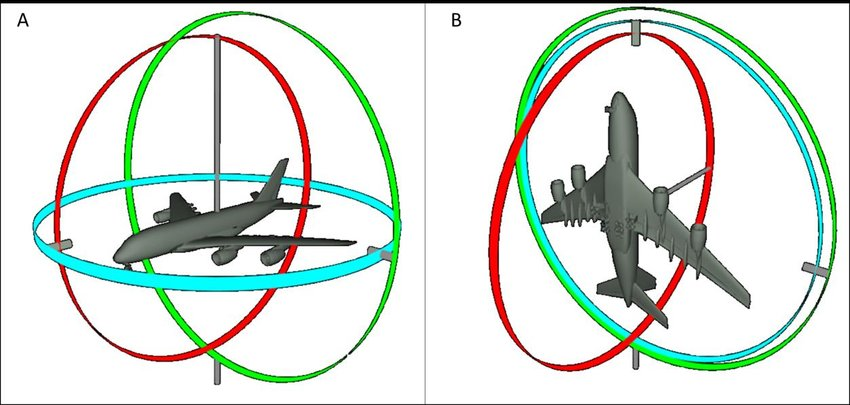
\includegraphics[width=10cm]{papers/clifford/Bilder/ReihenfolgeGimbal.png}
	\caption{Das Gimbal Lock tritt ein, wenn zwei Drehachsen in der gleichen Ebene liegen. Dies ist im rechten Bild bei der grünen und blauen Achse der Fall. Der rote Kreis würde sich an der oberen Halterung genau in die gleiche Richtung drehen, wie der grüne Kreis an der unteren Halterung. Man verliert somit eine Drehrichtung.}
	\label{BildReihenfolgeGimbal}
\end{figure}

\subsection{Gimbal-Lock}
Ein weiterer Nachteil der Eulerschen Winkel ist das Gimbal-Lock. Es entsteht dann, wenn zwei Ringe Deckungsgleich übereinander gedreht werden, wie man im Bild \eqref{BildReihenfolgeGimbal} sieht. Dabei verliert das Gimbal eine Drehrichtung, da der äussere und Innere Ring nun die gleiche Drehrichtung besitzen. Dies kann beispielsweise Probleme bei Spielen bei der Berechnung der Interpolation führen. Man hat dies bei älteren Spielen wie im Bild \ref{BildGimbalLock} dann gesehen, wenn plötzlich Gliedmassen bei den Spielermodellen in unnatürliche Richtungen gesprungen sind.

\begin{figure}
	\centering
	\includegraphics[width=10cm]{papers/clifford/Bilder/GimbalLock.png}
	\caption{Interpolationsfehler durch Gimbal-Lock}
	\label{BildGimbalLock}
\end{figure}
%
% teil3.tex -- Beispiel-File für Teil 3
%
% (c) 2020 Prof Dr Andreas Müller, Hochschule Rapperswil
%
\section{Fazit}
\rhead{Fazit}

Die geometrische Algebra ist dafür ausgelegt, geometrische Operationen, wie die Spiegelung oder Drehung, einfach zu beschreiben. Dadurch kann sie als gute Alternative zu der linearen Algebra angewendet werden, um grafische Probleme zu lösen. Sie kann zudem zum Verständnis der drehenden Eigenschaften der komplexen Zahlen und Quaternionen beitragen und die Zusammenhänge zwischen den komplexen Zahlen und den Quaternionen zeigen.

\printbibliography[heading=subbibliography]
\end{refsection}
